\documentclass[aspectratio=169]{beamer}

\usepackage[utf8]{inputenc}
%\usepackage{latexsym}
\usepackage{graphicx}
\usepackage{mathptmx}
\usepackage{amsmath}
%\usepackage{amsfonts}
\usepackage{amssymb}
%\usepackage{amsthm}
\usepackage{amsopn}
%\usepackage{amsbsy}
\usepackage{algorithmic}
\usepackage{bm}
\usefonttheme[onlymath]{serif}

% Get checkmark logo
\usepackage{pifont}
\newcommand{\cmark}{\ding{51}}
\newcommand{\xmark}{\ding{55}}
% Get \lee and \gee commands
\newcommand{\cX}{\mathbf{\mathcal{X}}}
\newcommand{\cY}{\mathbf{\mathcal{Y}}}
\newcommand{\vu}{\mathbf{u}}
\newcommand{\vv}{\mathbf{v}}
\newcommand{\vx}{\mathbf{x}}
\newcommand{\vy}{\mathbf{y}}
\newcommand{\nub}{\mathbf{\nu}}
\newcommand{\vC}{\mathbf{C}}
\newcommand{\vF}{\mathbf{F}}
\newcommand{\vG}{\mathbf{G}}
\newcommand{\vS}{\mathbf{S}}
\newcommand{\vO}{\mathbf{O}}
\newcommand{\si}{{(i)}}
\newcommand{\sj}{{(j)}}
\newcommand{\lee}{\leqq}
\newcommand{\gee}{\geqq}
\DeclareMathAlphabet{\mathcal}{OMS}{cmsy}{m}{n}

\usepackage[english]{babel}
\usepackage[utf8]{inputenc}

% AMSLaTeX packages
\usepackage{amsthm}
\usepackage{amsmath}
\usepackage{amsfonts}
\usepackage[algoruled]{algorithm2e}

\usetheme{default}
\useoutertheme{default}
% we want to use images
\usepackage{graphicx}
\usepackage{movie15}
\usepackage{hyperref}

% table relates packages
\usepackage{booktabs}
\usepackage{multirow}
% pick a font
\usepackage{palatino}           
% \usepackage{times}
\usepackage{tikz}
\usetikzlibrary[positioning,arrows,decorations.pathmorphing,backgrounds,fit,calc]
% \AtBeginSection[]  % "Beamer, do the following at the start of every section"
% {
%   \begin{frame}<beamer> 
%     \frametitle{Outline} % make a frame titled "Outline"
%     \tableofcontents[currentsection]  % show TOC and highlight current section
%   \end{frame}                    
% }

% \AtBeginSubsection[]
% {
%   \begin{frame}
%     \frametitle{Outline}
%     \tableofcontents[currentsection,currentsubsection]
%   \end{frame}
% }

\AtBeginSection[]
{
   \begin{frame}
       \frametitle{Outline}
       \tableofcontents[currentsection]
   \end{frame}
}

\newcommand{\ebox}[1][1em]{\framebox[#1]{\phantom{M}}}

\setlength\arraycolsep{1.4pt}% some length

%gets rid of navigation symbols
\setbeamertemplate{navigation symbols}{}

%gets rid of bottom navigation bars
\setbeamertemplate{footline}[page number]{}
\setbeamertemplate{headline}{}


\usebackgroundtemplate{\includegraphics[width=\paperwidth]{../templates/NormalANLBlue}}
% Title Information
\title{Surrogate Modeling of Simulations for Multiobjective Optimization Applications}
\author{Tyler~Chang and Stefan~Wild}
\date{July, 2021}
\institute{Mathematics and Computer Science Division\\
Argonne National Laboratory}

\begin{document}

\setbeamertemplate{footline}{}
{
\usebackgroundtemplate{\includegraphics[width=\paperwidth]{../templates/TitleANLBlue}}
\frame{\titlepage}
}

\setbeamertemplate{footline}[page number]{}

% FRAME: overview
\begin{frame}
  \frametitle{Outline}
  \tableofcontents
\end{frame}

% Intro section on the problem background
\section{Introduction and Motivation}

% Some basics and notation
\subsection{Notation}
\begin{frame}{Basic Notations and Terminology}
\begin{columns}
\begin{column}{.42\textwidth}
\includegraphics[width=\textwidth]{feasible_design.eps}\\
\centering{\it Design space}
\end{column}
\begin{column}{.15\textwidth}
\begin{center}
{\tiny
Objective Functions\\
}
$\xrightarrow{\hspace*{2cm}}$
\end{center}
\end{column}
\begin{column}{.42\textwidth}
\includegraphics[width=\textwidth]{convex_pareto.eps}\\
\centering{\it Objective space}
\end{column}
\end{columns}
\end{frame}

%\begin{frame}{Some more Notation}
%\begin{itemize}
%\item {\it Nondominated} is a property of a subset of the feasible objective
%space $\cY$;
%\item $\vF(\vx^{(1)}) \leq \vF(\vx^{(2)})$ if $\vF(\vx^{(1)})$ is
%componentwise less than or equal to $\vF(\vx^{(2)})$,
%with strict inequality in at least one component, and $\vF(\vx^{(1)})$ is
%said to {\it dominate} $\vF(\vx^{(2)})$;
%\item 
%If $\vF(\vx^*)$ satisfies $\vF(\vx) \not\leq \vF(\vx^*)$ for all
%$\vx \in \Omega \subset \cX$, then $\vF(\vx^*)$ is nondominated
%in $\vF(\Omega) \subset \cY$;
%\item $F(x)$ nondominated in $\cY \iff$ $F(x)$ is Pareto optimal.
%\end{itemize}
%\end{frame}
%
%\begin{frame}{Problem Class}
%Here we consider the problem class
%$$
%\min_{\vx\in{\cX}} \vF(\vx).
%$$
%\begin{itemize}
%\item $\cX \subset \mathbb{R}^d$;
%\item $\cX$ has upper/lower bounds (hard constraints);
%\item $\cX$ may also involve some nonlinear soft constraints, characterized
%by {\it constraint functions} $\vG(\vx) \leqq 0$;
%\item and both $\vF$ and $\vG$ may depend on one or more computationally
%expensive simulations.
%\end{itemize}
%\end{frame}

% Simulations
\subsection{The Simulation Function}
\begin{frame}{Adding the Simulation}
\begin{columns}
\begin{column}{.35\textwidth}
\includegraphics[width=\textwidth]{feasible_design.eps}\\
\centering{\it Design space}
\end{column}
\begin{column}{.11\textwidth}
\begin{center}
{\scriptsize
Simulations\\
}
$\xrightarrow{\hspace*{1.5cm}}$
\end{center}
\end{column}
\begin{column}{.08\textwidth}
\begin{center}
{\Huge $\mathcal{S}$}
\end{center}
\end{column}
\begin{column}{.11\textwidth}
\begin{center}
{\scriptsize
Objectives\\
}
$\xrightarrow{\hspace*{1.5cm}}$
\end{center}
\end{column}
\begin{column}{.35\textwidth}
\includegraphics[width=\textwidth]{convex_pareto.eps}\\
\centering{\it Objective space}
\end{column}
\end{columns}
\end{frame}

\begin{frame}{The Simulation Functions}
The simulations are denoted by a vector-valued function
$$\vS : \cX \rightarrow {\bf \cal S}.$$
Then the objective becomes
$$\vF : \cX, {\bf \cal S} \rightarrow {\cal Y},
\qquad \min_{\vx\in\cX}\vF(\vx, \vS(\vx))$$
and the constraint becomes
$$\vG : \cX, {\bf \cal S} \rightarrow \mathbb{R}^p,
\qquad \vG(\vx, \vS(\vx)) \leqq 0.$$
\end{frame}

\begin{frame}{Opening the Blackbox}
Our research question:\\

\bigskip

{\bf \large Can we take advantage of the simulation structure when the
objective $\vF$ and constraints $\vG$ are nice {\it algebraic functions} of
simulation outputs?}

\begin{itemize}
\item What (if anything) do we gain from modeling/evaluating $\vS$
separately from $\vF$/$\vG$?
\end{itemize}
\end{frame}

\section{PARMOO}
\subsection{Python Structure}

\begin{frame}{PARMOO}
\begin{itemize}
\item PARMOO is a Python library for parallel
multiobjective simulation optimization
\item One of the features of PARMOO is to handle simulations separately
from objectives
\begin{itemize}
\item Evaluate sims in $\vS$ in parallel
\item Model outputs of $\vS$, and compose with $\vF$ and $\vG$
\item Identify designs $\vx$ at which to evaluate sims $\vS$
\end{itemize}
\end{itemize}
\end{frame}

\begin{frame}{PARMOO continued}
\includegraphics[width=0.9\textwidth]{algorithm-chart.pdf}
\end{frame}

\subsection{Algorithmic Components}
\begin{frame}{PARMOO Response Surface Model}
\begin{columns}
\begin{column}{.4\textwidth}
\begin{itemize}
\item Global Search
\begin{itemize}
\item {\bf Latin hypercube search}
\item Global optimization (TBD)
\end{itemize}
\item Global surrogate
\begin{itemize}
\item {\bf Gaussian RBF}
\item Polynomial model (TBD)
\item Triangulation (TBD)
\end{itemize}
\item Optimizers
\begin{itemize}
\item Random search
\item {\bf GPS direct search polling}
\item SGD (TBD)
\item Quasi-Newton (TBD)
\end{itemize}
\end{itemize}
\end{column}
\begin{column}{.58\textwidth}
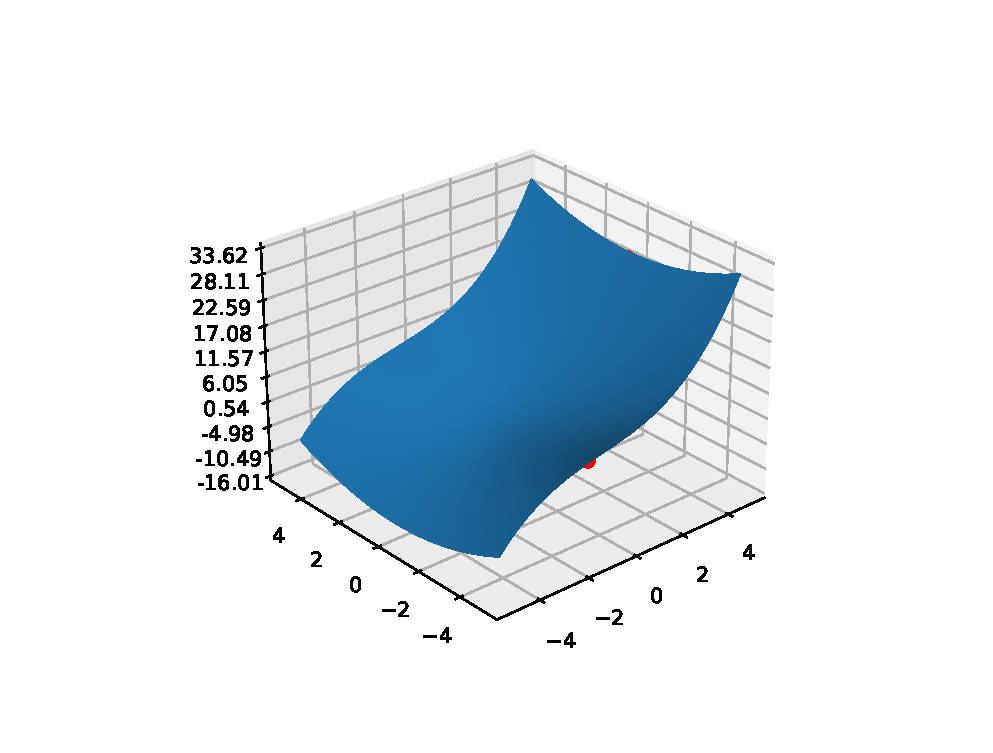
\includegraphics[width=\textwidth]{response_surface.eps}
\end{column}
\end{columns}
\end{frame}

\begin{frame}{PARMOO Acquisition}
\begin{columns}
\begin{column}{.6\textwidth}
\begin{itemize}
\item Uniform random weights
\item {\bf Fixed weights}
\end{itemize}
\end{column}
\begin{column}{.35\textwidth}
\includegraphics[width=\textwidth]{weights.eps}
\end{column}
\end{columns}
\pause
\begin{columns}
\begin{column}{.6\textwidth}
\begin{itemize}
\item {\bf Pick random target in the convex hull of nondominated pts,
and improve it}
\item Other TBD
\end{itemize}
\end{column}
\begin{column}{.35\textwidth}
\includegraphics[width=\textwidth]{set_target.eps}
\end{column}
\end{columns}
\end{frame}

\section{The Fayans EDF Problem}
\subsection{Problem Description}
\begin{frame}{The Fayans EDF Model}
As an example, consider the problem of fitting $9$ different observable
types for the Fayans EDF model:
\begin{columns}
\begin{column}{0.48\textwidth}
\begin{itemize}
\item Binding energy;
\item Charge radius;
\item Diffraction radius;
\item Surface thickness;
\item Neutron single-level energy;
\end{itemize}
\end{column}
\begin{column}{0.48\textwidth}
\begin{itemize}
\item Proton single-level energy;
\item Differential Radii;
\item Neutron pairing gap; and
\item Proton pairing gap.
\end{itemize}
\end{column}
\end{columns}
\end{frame}

\begin{frame}{Fitting the Fayans Model}
Find parameters $\vx \in \mathbb{R}^{13}$ so that the Fayans model
$M\left(\nub;\vx\right)$ agrees with data $(\nub_{t,i},d_{t,i})$:
$$
M\left(\nub_{t,i};\vx\right) \approx d_{t,i} \qquad i=1,\ldots, n_t;
\qquad t=1,\ldots, 9,
$$

\medskip

We have the simulation:
$$
S_{t,i}(\vx) = M\left(\nub_{t,i};\vx\right) - d_{t,i}
\qquad i=1,\ldots, n_t;
\qquad t=1,\ldots, 9
$$
\begin{itemize}
\item $m = \sum_{t=1}^9 n_t = 198$ total sim outputs
\end{itemize}

\vfill

{\tiny 
R.~Bollapragada, M.~Menickelly, W.~Nazarewicz, J.~O'Neal, P.G.~Reinhard, and S.M.~Wild. Optimization and supervised machine learning methods for fitting numerical physics models without derivatives. Journal of Physics G: Nuclear and Particle Physics 48(2), 2020.}\par

\end{frame}

\begin{frame}{The Fayans Multiobjective Optimization Problem}
The problem of fitting the Fayans EDF is formulated as
$$
\min_{\vx}\sum_{t=1}^9 \frac{1}{\sigma_t}F_t(\vx)
$$
where
$$
F_t(\vx) =  \sum_{i=1}^{n_t} S_{t,i}(\vx)^2,
\qquad t=1,\ldots, 9
$$
\begin{itemize}
\item $\sigma_t$ is the standard error -- errors in
measurement and model accuracy
\item The correct values of $\sigma_t$ are unknown
\end{itemize}
To find $\sigma_t$, solve:
$$\min_{\vx} (F_1(\vx), \ldots, F_9(\vx))$$
\end{frame}

\subsection{Theoretical Benefits}
\begin{frame}{Sum-of-squares Structure}
\begin{columns}
\begin{column}{0.6\textwidth}
Problem has a sum-of-squares structure to exploit:
$$
F_t = \sum_{i=1}^{n_t}S_{t,i}(\vx)^2
$$
\end{column}
\begin{column}{0.4\textwidth}
\begin{center}
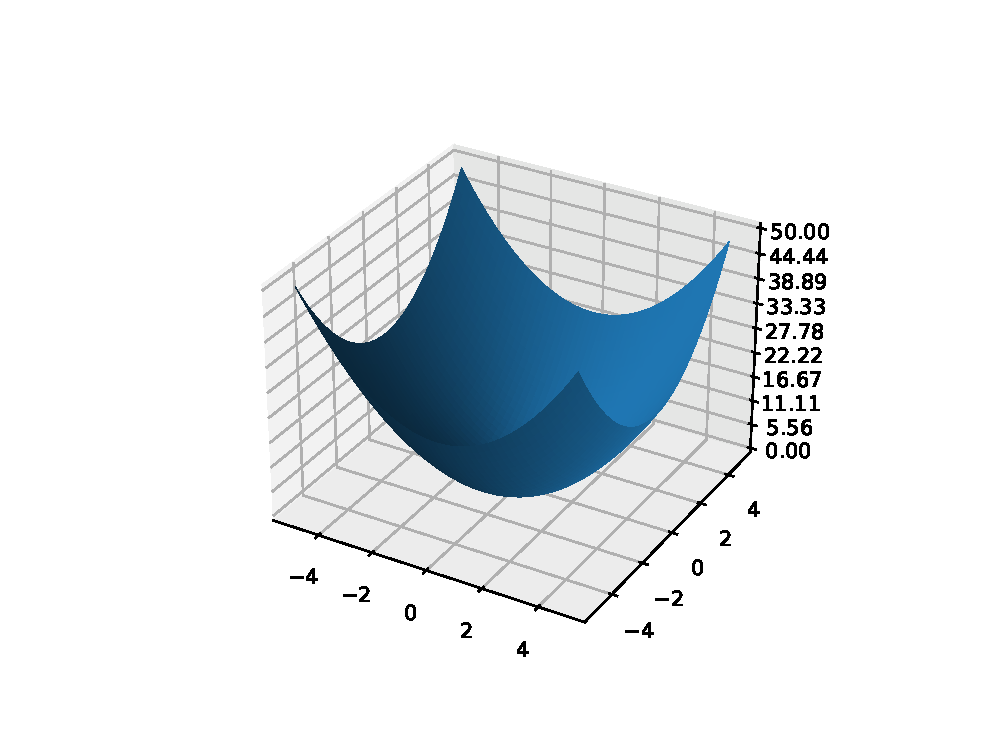
\includegraphics[width=0.8\textwidth]{quad.eps}
\end{center}
\end{column}
\end{columns}
\begin{itemize}
\item Use {\it fully linear models} to approximate $S_{t,i}$
(1st-order approx)
\item 
Pushing $\nabla S_{t,i}(x)$ through $F_t$ gives approximation to
the Hessian $\nabla^2 F_t(x)$ $^\dagger$ (2nd-order approx)
\item
Higher-order surrogate approximation
$\Rightarrow$ better surrogate optimization, right?
\end{itemize}

\vfill

{\tiny \it $\dagger$
H.~Zhang, A.R.~Conn, and K.~Scheinberg.
A derivative-free algorithm for least-squares minimization.
SIAM Journal on Optimization 20(6), 2010.

}

\end{frame}

\begin{frame}{What could go wrong?}
Not so fast!

\bigskip

\begin{itemize}
\item No single converging sequence $\Rightarrow$ No asymptotic model
convergence
\item Improved model order could be dominated by a decrease in smoothness
\end{itemize}

\bigskip

Is modeling $S_{t,i}(\vx)$ a good idea in practice?

Do we gain anything for the Fayans EDF calibration problem?
\end{frame}

\section{Experiments}
\subsection{Reduced Difficulty Problem}

%\begin{frame}{The Surrogate Problem}
%To save compute time, here we consider the surrogate errors
%${\hat S}_{t,i}(\vx) \approx S_{t,i}(\vx)$
%\begin{itemize}
%\item Uses inverse-distance weighting on $k=14$ ($=n+1$) nearest neighbors;
%\item 52,079 $\varepsilon$-unique data points extracted from the data set
%of {\it Bollapragada et al.}, with higher density around certain Pareto
%minima
%\item Also, we are not interested in solutions that are very far away
%from the minimizer of $\sum S_{t,i}(\vx)^2$ (in {\it Bollapragada et al.})
%so we add constraints
%\begin{itemize}
%\item Sum-of-squared binding energies ($F_1$) $< 804$;
%\item Sum-of-squared charge radii ($F_2$) $< 1510$;
%\item Sum-of-squared diffraction radii ($F_3$) $< 579$;
%\item Sum-of-squared surface thicknesses ($F_4$) $< 180$;
%\item Sum-of-squared neutron single-level energies ($F_5$) $< 189$;
%\item Sum-of-squared proton single-level energies ($F_6$) $< 53.1$;
%\item Sum-of-squared differential radii ($F_7$) $< 10$;
%\item Sum-of-squared neutron pairing gaps ($F_8$) $< 10$;
%\item proton pairing gaps ($F_9$) $< 170$.
%\end{itemize}
%\end{itemize}
%\end{frame}

\begin{frame}{3-objective variation}
Reduce problem difficulty by bringing down to 3 objectives:
\begin{itemize}
\item Binding energy ({\bf sum of 63 squared errors});
\item Std radii (charge radius + diffraction radius, {\bf sum of 80 squared errors});
\item Other (all other quantities of interest, {\bf sum of 55 squared errors});
\end{itemize}
\end{frame}

\begin{frame}{The Substitute Problem}
To save compute time, we use a substitute problem
$${\hat S}_{t,i}(\vx) \approx S_{t,i}(\vx)$$
\begin{itemize}
\item 
Based on 52,079 $\varepsilon$-unique data points
(from {\it Bollapragada et al.})
\item Uses inverse-distance weighting on $k=14$ ($=n+1$) nearest neighbors;
\item We are not interested in solutions that are very far away
from the minima of $\sum S_{t,i}(\vx)^2$ found by {\it Bollapragada et al.}:
\begin{itemize}
\item Sum-of-squared binding energies ($F_1$) $< 804$;
\item Sum-of-squared std radii ($F_2$) $< 2090$;
\item Sum-of-other-squares ($F_3$) $< 613$.
\end{itemize}
\end{itemize}
\end{frame}

\subsection{Embedding Fayans EDF in PARMOO}

\begin{frame}{Embedding Fayans EDF in PARMOO}
\begin{columns}
\begin{column}{0.7\textwidth}
\begin{itemize}
\item 2000 pt LHS search
\item Gauss RBF surrogates
\item 10 total acquisition functions ($\Rightarrow$ 10 sim evals per iteration)
\begin{itemize}
\item 9 Improve random acquisition
\item 1 fixed (equal) weights acquisition function
\end{itemize}
\item GPS polling optimizer
\item 10,000 sim budget (-2000 LH search) $\Rightarrow$ 800 iterations
\end{itemize}
\end{column}
\begin{column}{0.29\textwidth}
\includegraphics[width=\textwidth]{solns.pdf}\\
\vskip -30pt
\begin{center}
{\it Bollapragada et al.}
minimized sum-of-squares for all 198 errors, and found 2 solution types (above)
\end{center}
\end{column}
\end{columns}
\end{frame}

\begin{frame}{Two Problem Variations}
Recall, our goal is to determine whether anything is gained by modeling
the individual errors instead of the sum-of-square errors:
\pause
\begin{enumerate}
\item Simulations produce a 198-dimensional error vector
\begin{itemize}
\item $m=198$ surrogate outputs, $3$ objectives = sum-of-squared sim outs
\item Surrogates applied to each error, so sum-of-squares structure
is exploited {\huge \color{green} \cmark}
\end{itemize}
\pause
\item Simulations given as 3-dimensional sum-of-squared error objective vector
\begin{itemize}
\item Objectives are given as the identity function on each simulation
output
\item Surrogates applied to true objectives, so sum-of-squares structure
is not exploited {\huge \color{red} \xmark}
\end{itemize}
\end{enumerate}
\end{frame}

\subsection{Results and Conclusions}
\begin{frame}{Full Solution}
Full solution set:
Nondominated objective values from original 52,079 data points
+ 100,000 new evaluations
\begin{columns}
\begin{column}{0.5\textwidth}
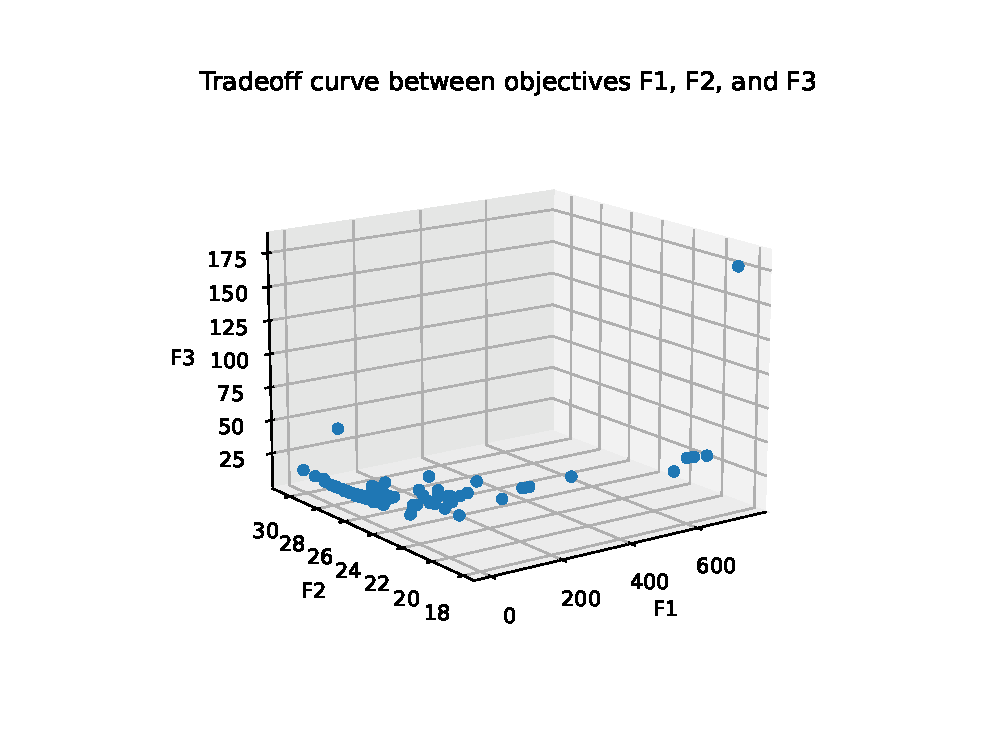
\includegraphics[width=\textwidth]{soln_1.eps}
\end{column}
\begin{column}{0.5\textwidth}
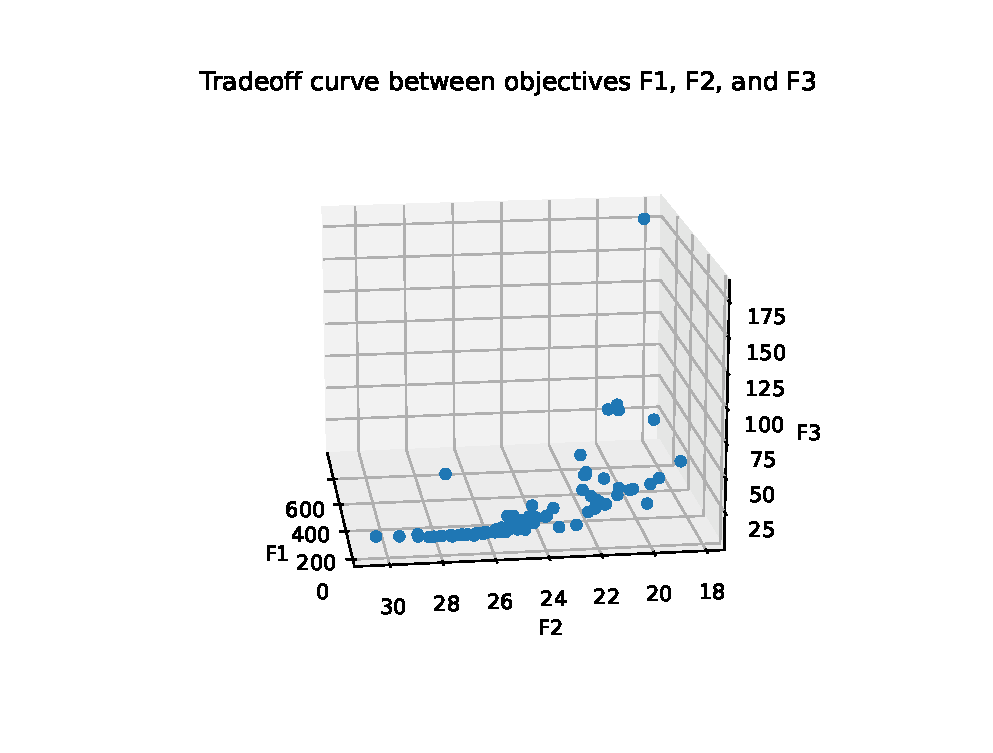
\includegraphics[width=\textwidth]{soln_2.eps}
\end{column}
\end{columns}
\end{frame}

\begin{frame}{Performance Measures}
Minimum sum-of-squares (measures convergence of one fixed AcquisitionFunction)
\begin{itemize}
\item Note: This is the only metric expected to reach asymptotic convergence
rate
\end{itemize}
\begin{center}
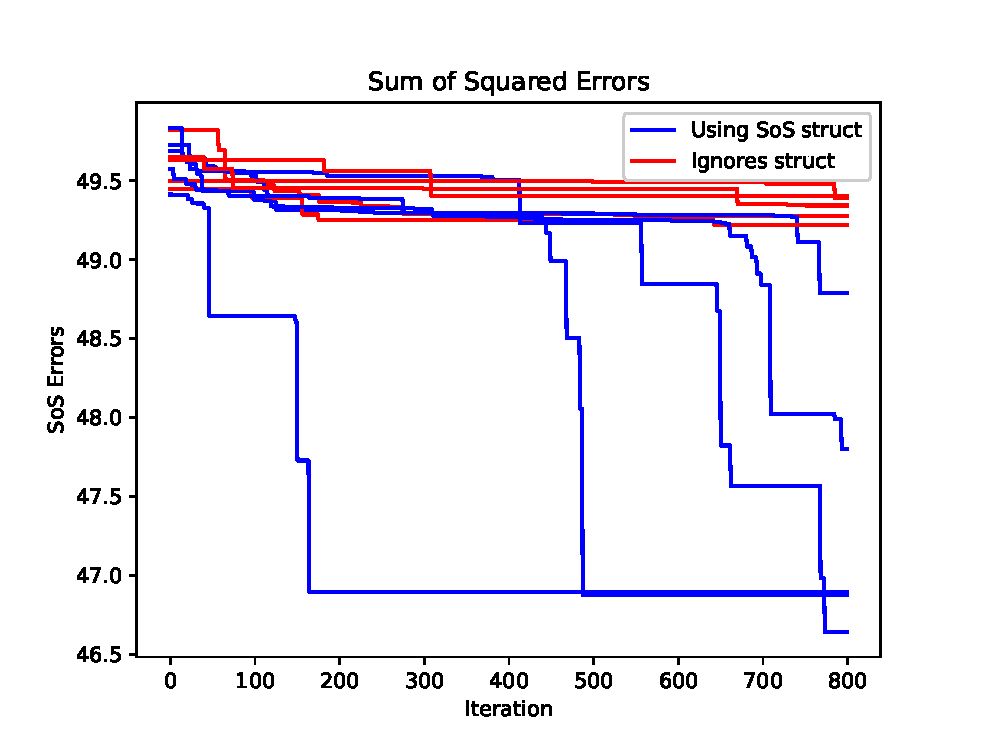
\includegraphics[width=0.5\textwidth]{sos_error.eps}
\end{center}
\end{frame}

\begin{frame}{Performance Measures}
Hypervolume indicator (proportion of hypercube between upper bounds
and the origin that is dominated by each solution set)
\begin{center}
\includegraphics[width=0.5\textwidth]{hv_1.eps}
\end{center}
\end{frame}

\begin{frame}{Conclusions}
\begin{itemize}
\item The sum-of-squares structures is successfully exploited in this problem
by modeling simulations separately from objectives/constraints
\item Effective for both accelerating convergence to a single Pareto point
and for finding ``isolated'' Pareto points
\end{itemize}
\pause
Future work
\begin{itemize}
\item Investigate the full 9 objective problem
\item Add an acquisition function option for setting adaptive targets on the
Pareto front
\item Continue to improve PARMOO/add other surrogates and better optimizers
\item Investigate other structures (such as heterogeneous objectives)
\end{itemize}
\end{frame}

\begin{frame}
  \frametitle{Questions}
  \tableofcontents
  \bigskip

\par
{\tiny This material is based upon work supported by the U.S. Department of Energy, Office of Science, Office of Advanced Scientific Computing Research, SciDAC program under contract number DE-AC02-06CH11357.}\par

\end{frame}
\end{document}
